% !Mode:: "TeX:UTF-8"%確保文檔utf-8編碼
%新加入的命令如下: reduline showendnotes 
%新加入的环境如下:solution solutionorbox solutionorlines solutionordottedlines

\documentclass[12pt,twoside]{exam}
\newlength{\textpt}
\setlength{\textpt}{12pt}

\usepackage{teachingplan}


%写上答案或者不写上答案%1  
%\printanswers  


%讲知识点然后测试,测试通过继续下一个知识点。不通过给予小提示,然后继续测试,如果通过那么通过,如果还是不会做,那么继续讲解知识点,并讲解这个题目,然后重新给出一个题目重新测试。

%如果有精力,后面再准备一套中考真题。

%\excludecomment{knowledge}
\includecomment{knowledge}
%\excludecomment{Aquestions}
\includecomment{Aquestions}


\begin{document}
\begin{coverpages}
\title{运动的描述}
\author{德山书生}
\maketitle
\tableofcontents
\end{coverpages}
\begin{knowledge}
\begin{flushright}
\begin{notecard}{16em}
\ttfamily 
敢于承认自己的无知也是一种智慧。
\end{notecard}
\end{flushright}
\section{长度的测量}
测量需要有标准,测量某个物理量时用来进行比较的标准量叫做单位。为了交流的方便,国际计量组织制定了一套国际统一的单位,叫国际单位制。

长度的测量工具有:刻度尺、米尺、皮卷尺、游标卡尺、激光测距仪等。

\subsection{长度的单位}
长度的国际单位是\answerline*[米],常用的国际单位及其符号有:千米(km)、分米(\answerline*[dm]) 、厘米(cm)、毫米(\answerline*[mm])、微米(\si{\micro m}
)、纳米(\answerline*[nm])。

\leftnote{问学生换算}

\textbf{问题:}1nm=\answerline*[\num{d7}]\si{cm} ,1mm=\answerline*[\num{d3}]\si{\micro m}

\subsection{长度的生活经验}
有些题目考学生对长度或者其他物理量的生活感知认识,这些题目并不难,但需要学生仔细认真。

\textbf{(2013河南,8,2分)}为了解自己的身体状况,小丽做了一些测量,其中记录\dotuline{错误的}是(\answerline*[A])

\begin{oneparchoices}
\choice 身高16m
\choice 质量40kg
\choice 体温37\si{\degreeCelsius}
\choice 1min心跳75次
\end{oneparchoices}


\subsection{刻度尺}
\subsubsection{使用刻度尺注意事项}
\begin{enumerate}
\item[①] 注意刻度标尺的零刻度线、最小\answerline*[分度值]和量程。
\item[②] 测量时尺要沿着所测长度,尽量靠近被测物体,不用磨损的零刻度线。
\item[③] 读数时视线要与尺面\answerline*[垂直],在精确测量时要\dotuline{估读}到分度值的下一位。
\item[④] “记”,测量值由数字和\answerline*[单位]组成,最末一位是\answerline*[估读]值,包括估读值在内的测量值称为有效数字。
\end{enumerate}

\subsubsection{分度值}
长度测量的精确程度是由刻度尺的分度值决定的,要根据需要达到的精确度选择刻度值和量程合适的刻度尺。比如只是测量身高,用分度值\answerline*[cm]的刻度值就可以了,而测量窗户的长度,则要用分度值是\answerline*[mm]的刻度尺。

\textbf{问题:}用最小刻度值是$0.1$毫米的尺子去测量某钢丝的直径,下面是几个同学的记录,其中有效数字错误的是(\answerline*[C])

\begin{oneparchoices}
\choice 0.52毫米
\choice 0.53毫米
\choice 0.518毫米
\choice 0.052厘米
\end{oneparchoices}


\subsubsection{长度的估读}
\leftnote{视线?}单位?估读?

\textbf{问题:}某同学以铅笔长为单位长,测得一桌子的长度为单位长的5.6倍,则桌子的长应记作\answer[70pt]{5.6铅笔长},其中准确值为\answerline*[5铅笔长],估计值为\answer[70pt]{0.6铅笔长}。


\textbf{问题:}用刻度尺测出桌子的长度为1.243m,所用的刻度尺的分度值是\answerline*[cm],测量的准确程度达到\answerline*[1cm]。

\textbf{(2013湖北黄冈,34,3分)}图甲圆柱体直径为\answerline*[0.90]cm;图乙是游码在天平标尺上的位置,其表示的质量为\answerline*[1.2]g;图丙温度计的读数是\answerline*[9]\si{\degreeCelsius}。

\newpage
\vspace*{40pt}
\noindent
\begin{minipage}{\textwidth}
\begin{minipage}[c][6cm][c]{0.78\textwidth}
\begin{figure}[H]
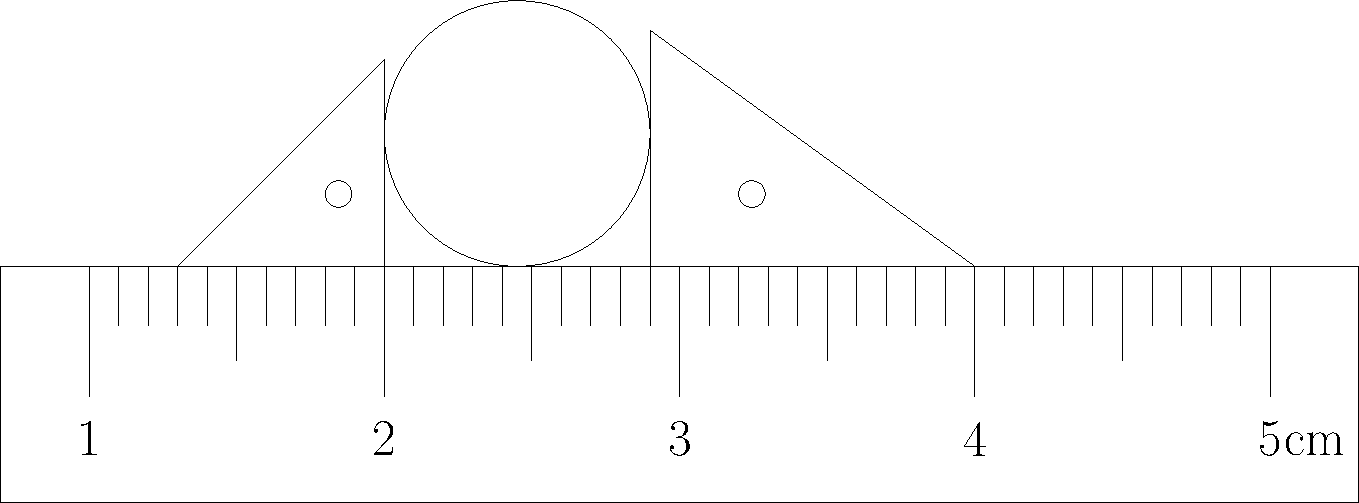
\includegraphics[width=\linewidth]{figures/2013湖北黄冈34甲.pdf} 
\caption{甲}
\end{figure}
\begin{figure}[H]
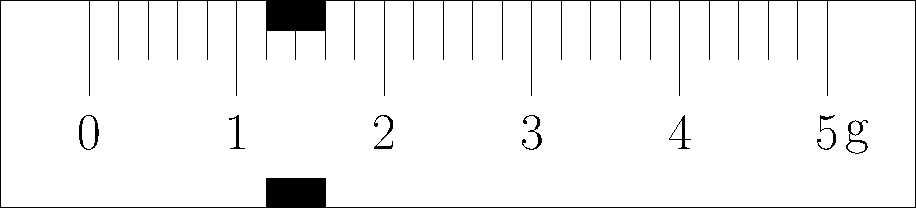
\includegraphics[width=\linewidth]{figures/2013湖北黄冈34乙.pdf} 
\caption{乙}
\end{figure}
\end{minipage}\hfill
\begin{minipage}[c][6cm][c]{0.2\textwidth}
\begin{figure}[H]
\centering
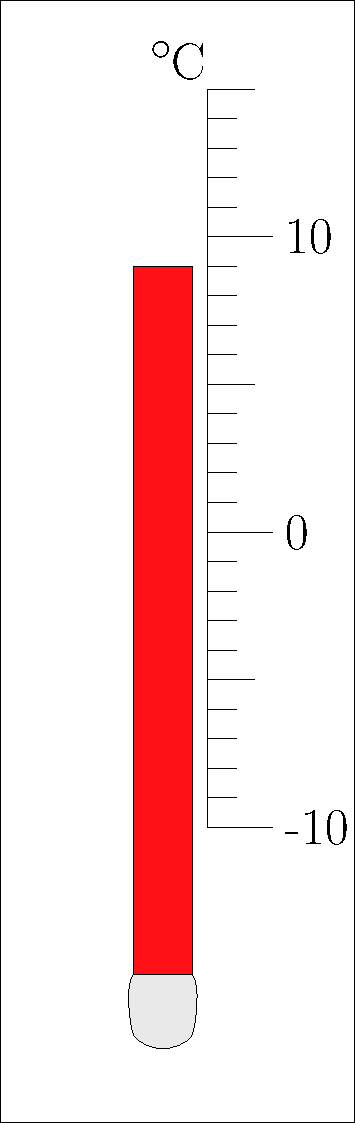
\includegraphics[width=0.9\linewidth]{figures/2013湖北黄冈34丙.pdf} 
\caption{丙}
\end{figure}
\end{minipage} 

\end{minipage} 

\vspace{45pt}


\subsection{初中物理对估读的要求}
初中物理大纲要求\uwave{长度的测量}是要估读一位的,其他物理量\uwave{都}不做要求。


\subsection{关于误差的讨论}
用测量仪器测定待测物理量所得的数值叫测量值,任何一个物理量都有一个客观大小,这个客观值叫做真实值,真实值是不可测的。测量值和真实值之间的偏差叫做误差,我们不能消灭误差,但应尽量减小误差。误差的产生与测量仪器、测量方法、测量的人有关。

减少误差方法:多次测量求平均值、选用精密测量工具、改进测量方法,熟练实验技能等。

误差与错误区别:误差不是错误,错误不该发生能够避免,误差永远存在不能避免。


\textbf{问题:}小红想要知道从自己家到学校有多远的距离,于是她决定采用类比的方法。首先她知道学校的跑道有四百米,于是她进行了五次实验,实验的内容就是从跑道上走一圈统计所走的步数。所得结果如下:
\begin{table}[H]
\centering
\begin{tabular}{|p{8ex}|c|c|c|c|c|}
\hline 
实验次数 & 1 & 2 & 3 & 4 & 5 \\ 
\hline 
所用步数 & 884 & 857 & 853 & 871 & 884 \\ 
\hline 
\end{tabular} 
\end{table}
那么请问小红平均走一步的距离是多少?然后小红又测得从自己家走到学校需要走$8960$步。那么小红家到学校的距离是?

小红在这里进行了多次实验取平均值的方法,请问小红为什么要这么做?


\begin{solution}[10ex]
参考答案:平均一步距离约为:$0.46m$,小红家到学校的距离约为:$4121.6$米。小红多次实验取平均值是为了减少测量误差,让自己的测量值更准确。
\end{solution}



\subsection{测量距离的方法}
\subsubsection{直接拿尺子量}
这个不用多说了。

\subsubsection{累计法}
在生活中我们要测量某个微小的长度,可以采用将那个微小的长度累积变成一个很大的长度,这样再来测量。比如测量纸张的厚度我们可以先测量一本书的厚度,然后除以这本书包含的纸张数,这样我们就得到了这本书的一张纸的平均厚度(也就是n张纸$\times$每张纸的厚度=书的总厚度);比如铜线的直径,我们可以将这段铜线绕在圆铅笔上紧密绕很多圈,这样我们便可以求出细铜丝的直径了(也就是n圈$\times$细铜丝的直径=铜丝排布的总长度。)

此外还有用自行车测一段马路的长,可以先测出车轮的周长,然后计算自行车通过这段马路转了多少圈(这样马路的总长度=圈数n$\times$自行车的车轮周长。)

\textbf{(2012山东潍坊,23,5分)}蚊香生产者为了节约原料和用户使用方便,要根据蚊香的燃烧速度生产规格不同的各种蚊香。有一种蚊香如图所示,请你设计一个实验,测出该蚊香正常燃烧的速度。要求:
\begin{multicols}{2}
\begin{enumerate}
\item 写出所需要的器材
\item 说明测量方法
\end{enumerate}
\columnbreak
\hfill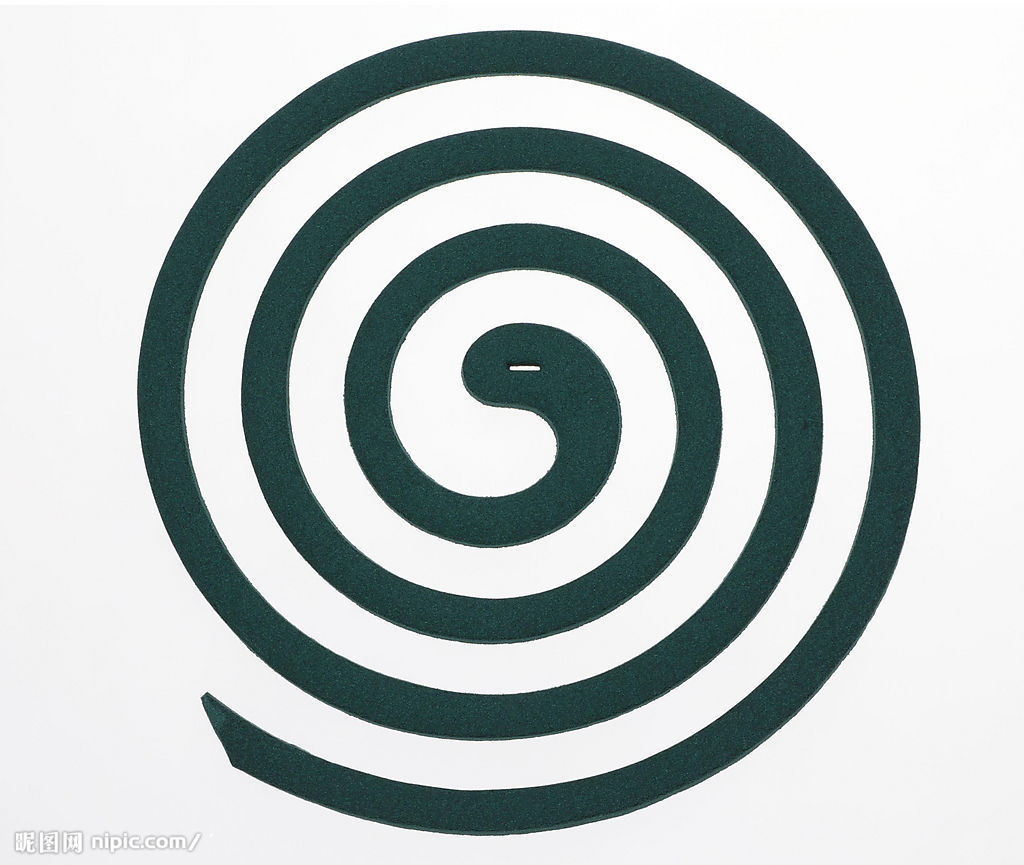
\includegraphics[scale=0.1]{figures/蚊香.jpg} 
\end{multicols}
\pagebreak
\begin{solutionorbox}[12ex]
器材:蚊香,细线,刻度尺,秒表,火柴(2分)\\
让细线和蚊香重合,测量细线的长度,然后根据速度公式$v=s/t$来计算。其他方法只要可行也可得分。
\end{solutionorbox}



\subsubsection{间接法}
\textbf{问题:}测量大楼或者高山的高度\\
小明想要测量某个大楼的高度,然后他拿了一根棍子,让这个棍子的影子正好落在大楼影子的末端重合。然后他测得这个一米长的棍子的影子长($l1$)1m,测得从棍子到大楼的距离($l2$)是304m。那么请问这座大楼有多高?

\usetikzlibrary{decorations.pathreplacing}

\begin{figure}[H]
\hfill
\begin{tikzpicture}[scale=0.5]
\newcommand{\sun}[2][]{
\begin{scope}[#1]
\def\sunr{#2}
\draw (0,0) circle (\sunr);

\foreach \angle in { 0,45,...,360 }{
\draw [rotate around={\angle:(0,0)}]
(\sunr+\sunr,0) -- +(\sunr,0);
}
\end{scope}
}

\draw (5,0) rectangle (6,5);

\draw (3,0) -- (3,3);

\draw (0,0) -- (10,0);
\draw[thick] (0,0) -- (10,10);

\sun[xshift=10cm,yshift=10cm,ultra thick]{0.2}

\draw[decorate,decoration={brace,amplitude=8},rotate=180,xshift=-3cm] (0,0) to node[below = 3mm] {$l1$} (3,0) ;

\draw[decorate,decoration={brace,amplitude=6},rotate=180,xshift=-8cm] (3,0) to node[below = 3mm] {$l2$} (5,0) ;

\end{tikzpicture}
\end{figure}

\subsubsection{速度法(根据$s=vt$)}
\textbf{问题:}激光测距仪\\
1969年7月21日阿波罗11号飞船的组员在月球上安置了复归反射器(如下图所示),可以将地球射出的激光平行返回到原射出点。这样就可以测得地球和月球之间的距离。这个实验的成果之一就是发现月球在以每年3.8厘米的速度远离地球。有一次测量从射出到受到返回的激光花了2.56秒,那么请问地球到月球的距离是\answer[80pt]{384000km}?(已知光速$c=3\times 10^8 m/s$)


\begin{figure}[H]
\hfill
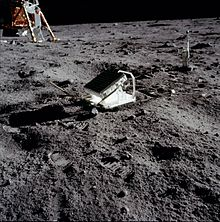
\includegraphics[scale=1.5]{Apollo_11_Lunar_Laser_Ranging_Experiment.jpg} 
\end{figure}



\subsubsection{三角法(测量大的距离)}
探险家汤姆破解了最新的藏宝图,藏宝图的密码是两个废弃的金字塔,金字塔A上垂直放一面镜子,对着下午4点钟时候的太阳光,宝藏就在反射光所指的方向;

金字塔B上也要垂直放一面镜子,对着早上9点钟时候的太阳光,宝藏就在放射光所指的方向。汤姆马上就找到宝藏的方法了。请问汤姆是怎么做到的?

\begin{fig}[0.8]{三角法寻宝}
\end{fig}


\section{时间的测量}
时间的测量工具有:秒表、手表等等。(生活中能够看时间的工具都能用来测量时间喽。)

时间的国际主单位是\answerline*[秒](s);常用的单位有小时(h)分(min)等。1h= 60min=360s。


\subsection{秒表的使用}
秒表的分度值是多少?幸运的是初中阶段除了长度需要估读其他都不需要估读,所以你读到达到多少秒就写多少秒喽。

那么什么是时间?\leftnote{别扯太远}

\subsection{计时的方法(周期性的事件)}
\subsubsection{生活中的时间}
比如以太阳周期性升起计时一天  。此外还有一年(叶子落下,花开花落),心跳等等。这些时间的生活经验也可能考对错题。


\subsubsection{更加精确的周期性事件}
单摆,电磁波的振动频率。(比如我们的日常用电是50Hz,也就是1s50个周期。这样一个周期就是1/50s,我们就可以用这个周期来计时。)


\subsubsection{速度法}
(根据$t=\frac{s}{v}$)


\section{运动的描述}
\subsection{机械运动}
物理学上把物体\answer[80pt]{位置的变化}称为机械运动。


\subsection{参照物}
在研究物体的机械运动时,需要明确是以哪个物体为标准,这个作为标准的物体叫\answerline*[参照物]。

(就坐火车或坐汽车的实际生活经验讲开去)

所以自然界一切物体都在运动,静止是相对的,我们观察同一物体是运动还是静止,取决于所选的\answerline*[参照物]。


\textbf{(2013广西南宁,1,2分) } 2012年11月23日,国产歼-15舰载机首次在航空母舰“辽宁号”上成功起降。如图所示,飞机起飞时,若说该飞机上的飞行员是静止的,所选的参照物是(\answerline*[B])

\begin{oneparchoices}
\choice 航母 
\choice 该飞行员驾驶的飞机
\choice 海水
\choice 航母上的工作人员
\end{oneparchoices}

\begin{linefig}[0.8]{2013广西南宁1}
\end{linefig}
\begin{multicols}{2}


\textbf{(2013山西,31,2分)}图是“辽宁号”航母指挥员正在用“走你”的动作指挥飞机起飞的情景。飞行员看到指挥员向后退去,是以\answerline*[飞机]为参照物,飞机\answerline*[逆]风(填“顺”或“逆”)时更容易起飞。
\columnbreak
\begin{linefig}{2013山西31}
\end{linefig}
\end{multicols}


\section{运动的快慢}
物体通过的路程和通过这段路程所需的时间的比值,称为物体在这段路程或这段时间内的\answerline*[速度]。

速度表示物体运动快慢的物理量,公式$v=s/t$,国际单位是米每秒(m/s)。

1m/s=3.6km/h(这个记住方便换算。)


\textbf{问题:}下列四个选项中,平均速度最大的是(\answerline*[B])
\begin{choices}
\choice 航模飞行器以11m/s的速度飞行 
\choice 汽车以50km/h的速度在公路上行驶
\choice 百米赛跑中运动员用10s时间跑完全程
\choice 从30m高出竖直下落到地面的物体用了2.5s
\end{choices}

\subsection{速度的生活常识}
人走路的速度约为3~4公里每小时,跑步的速度约为15公里每小时,自行车的速度约为30公里每小时,摩托车的速度约为五六十公里每小时,汽车的速度最快约为一百多公里每小时,一般火车的速度和汽车的速度差不多的,超过二百公里每小时的是动车。


\textbf{问题:}小汽车在高速公路上正常行驶,它的速度最接近(\answerline*[B])

\begin{oneparchoices}
\choice 3m/s
\choice 30m/s
\choice 300m/s
\choice 3000m/s
\end{oneparchoices}

\textbf{(2013贵州贵阳,15,2分)}据悉,全程约800km的贵(阳)广(州)高速铁路将于2014年建成通车,列车全程的行驶时间只需4h,则列车这段路程的平均速度为\answerline*[200]km/h。若仅考虑地理位置的关系, \leftnote{若学生不了解重力势能和动能,第二问可忽略。}同一列车从贵阳开到广州比从广州开到贵阳所消耗的能量要\answerline*[小](选填“大”或“小”)。



\subsection{平均速度}
匀速直线运动的特点是速度大小不变,方向不变。变速直线运动的速度大小改变,方向不变。只能用平均速度——也就是该物体走过的总路程除以总的时间(计算公式都是类似的,简单提一下即可。)

\textbf{(2013山东济南,18,2分)}如图为告诉摄影机拍摄的子弹射过柿子的照片\leftnote{这里可以简单提下瞬时速度的概念}。若子弹的平均速度是900m/s,则子弹穿过柿子的时间大约为(\answerline*[C])

\begin{multicols}{2}
\begin{choices}
\choice 0.1min
\choice 0.1s
\choice 0.1ms
\choice 0.1\si{\micro}s
\end{choices}
\columnbreak
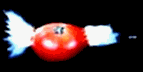
\includegraphics[scale=1]{figures/子弹穿过柿子.png} 
\end{multicols}

\textbf{(2013山东烟台,17,2分)}小明一家双休日驾车外出郊游,在汽车行驶的过程中,小明同学观察了一下速度及里程表盘如甲所示,此时汽车的行驶速度为\answerline*[80km/h]。汽车行驶了半个小时后,表盘的示数如图乙所示,那么这段时间内汽车行驶的平均速度为\answerline*[80km/h]。

\begin{multicols}{2}
\begin{linefig}[0.8]{2013山东烟台17甲}
\caption{甲}
\end{linefig}
\columnbreak
\begin{linefig}[0.8]{2013山东烟台17乙}
\caption{乙}
\end{linefig}
\end{multicols}


\subsection{距离-时间图}
我们在数学中学过一次函数,比如下面是描述一个物体的距离-时间图,你能从中看到什么?
\begin{fig}{路程-时间图}
\end{fig}


从0-2秒物体在做什么运动?从2-4秒是什么运动?走了多远的距离?速度是多少?从4-6秒是什么运动?走了多远的距离?速度是多少?整个过程又是什么运动?走了多远的距离?平均速度是多少?

\textbf{(2012上海,7,2分)[难]}甲、乙两物体同时同地同方向开始做匀速直线运动,甲的速度大于乙的速度,它们的s-t图象为下图所示a、b、c三条图线中的两条,运动5秒甲、乙间的距离大于2米,则(\answerline*[A])
\pagebreak
\begin{multicols}{2}
\begin{linefig}[0.9]{2012上海7}
\end{linefig}
\begin{choices}
\choice 甲的s-t图一定为图线a 
\choice 甲的s-t图可能为图线b  
\choice 乙的s-t图一定为图线c  
\choice 乙的s-t图可能为图线a
\end{choices}
\end{multicols}

\begin{multicols}{2}
\textbf{(2011黑龙江哈尔滨,39,2分)}甲、乙两辆汽车在水平路面上同时向东行驶,路程-时间图象如图所示,则甲车的速度是\answerline*[15]m/s;两车行驶过程中,若以甲车为参照物,乙车向\answerline*[西]运动。                      
\columnbreak
\begin{linefig}{2011黑龙江哈尔滨39}
\end{linefig}
\end{multicols}

\subsection{速度-时间图}
速度-时间图是描述一个物体运动速度和时间的关系图,下面这幅图你会看吗?
\begin{fig}{速度-时间图}
\end{fig}

在0-4秒是什么运动?4-6秒的时候A物体和B物体谁的速度快,各是多少?


\textbf{(2013辽宁沈阳,14,2分)}甲、乙两个物体同时从同一地点向西做直线运动,速度与时间关系如图所示。以甲为参照物,乙向\answerline*[东]做直线运动,经过6s甲乙两物体相距\answerline*[30]m。

\hfill
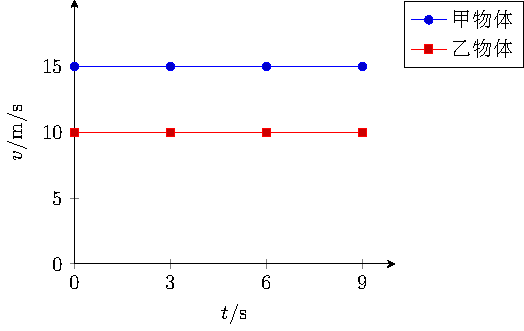
\includegraphics[scale=1]{figures/2013辽宁沈阳14.pdf} 


\textbf{(2010广东广州,13,3分)}甲、乙、丙三辆小车同时、同地向同一方向运动,它们运动的图象如图所示,由图象可知:运动速度相同的小车是\answerline*[甲]\\和\answerline*[丙];经过5s跑在最前面的小车是\answerline*[乙]。
\begin{multicols}{2}
\begin{linefig}{2010广东广州13-1}
\end{linefig}
\columnbreak
\begin{linefig}{2010广东广州13-2}
\end{linefig}
\end{multicols}


\section{总结}
现在我们已经学会了如何用\textbf{速度}这个概念来描述物体的运动的情况,其中涉及到了\uwave{长度},\uwave{时间},\uwave{参照物}等的概念。速度这一块大题主要以实验探究的形式展开。值得一提的是虽然初中并不讨论加速度这个概念,但常常有些题目实际上已经涉及到了。

\textbf{(2010湖北黄冈,23,3分)[难]}物理学中将物体在单位时间内速度的增加量定义为加速度。依据该定义,若某物体在$t$时间内速度从$v_1$增加到$v_2$,则加速度为{\large $\frac{v_2-v_1}{t}$}。现有一小球从静止开始以3\si{m/s^2}的加速度加速运动2s,则2s末小球的速度为(\answerline*[D])

\begin{oneparchoices}
\choice 0
\choice 2m/s
\choice 3m/s
\choice 6m/s
\end{oneparchoices}

最后我们来通过这些大题来检验一下自己对这一章的理解程度。

\textbf{(2011江西,23,8分)}某物理兴趣小组利用带有刻度尺的斜面、小车和数字钟“测量小车的平均速度”,如图所示,图中显示的是他们测量过程中的小车在甲、乙、丙三个位置及其对应时间的情形,显示时间的格式是“时:分:秒”。
\begin{linefig}{2011江西23-1}
\end{linefig}

(1)请你根据图示完成下表。

\begin{table}[H]
\resizebox{\linewidth}{!}{
\begin{tabular}{|c|c|c|c|}
 \hline 
 & 小车由甲至乙 & 小车由乙至丙 & 小车由甲至丙 \\ \hline
 路程 $s$/cm & 26 &  &  \\ \hline
 时间 $t$/s &  & 4  &  \\ \hline
 平均速度 $v$ (cm/s) &   &  & 15  \\ \hline
\end{tabular}
}
\end{table}

(2)分析表中数据,小车全程是做匀速运动吗?为什么?
\begin{solutionorbox}[12ex]
不是,从甲到乙的平均速度为$v_1=s_1/t_1=13cm/s$,从乙到丙的平均速度为$v_2=s_2/t_2=16cm/s$,由此可知小车全程不是匀速运动。
\end{solutionorbox}


\end{knowledge}





\begin{Aquestions}
\newpage
\section{题库A}
\begin{questions}
\question
妈妈用电动车送小明上学,途中妈妈提醒小明“坐好,别动!”。这个“别动”的参照物是(\answerline*[A])

\begin{choices}
\choice 电动车上的座位
\choice 路旁的树木
\choice 迎面走来的行人 
\choice 从旁边超越的汽车
\end{choices}


\question
小明坐在行驶的列车内,若说他是静止的,则所选择的参照物是(\answer[39pt]{A})\par
\begin{oneparchoices}
\choice 车窗
\choice 铁轨
\choice 路边的树
\choice 在车内走动的乘务员
\end{oneparchoices}


\question
一辆汽车沿平直的公路向西快速行驶,一个行人沿该公路的便道向西散步。以行人为参照物汽车(\answerline*[B])

\begin{choices}
\choice 向东运动
\choice 向西运动
\choice 静止不动
\choice 无法确定
\end{choices}


\question
机场周围不允许有鸟类飞行,以免撞毁飞机。这是因为(\answerline*[D])
\begin{choices}
\choice 以地面为参照物,鸟的速度非常大
\choice 以机场步行的人为参照物,鸟的速度非常大
\choice 以机场内的飞机为参照物,鸟的速度很大
\choice 以正在飞行的飞机为参照物,鸟的速度很大
\end{choices}


\question
甲、乙两位同学进行百米赛跑,假如把他们的运动近似看作匀速直线运动处理,他们同时从起跑线起跑,经过一段时间后他们的位置如下图所示,在图中分别作出在这段时间内两人运动路程$s$、速度$v$与时间$t$的图像,正确的是(\answerline*[B])

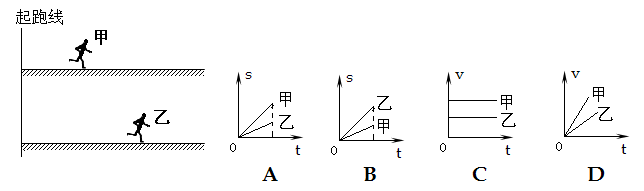
\includegraphics[scale=0.8]{figures/图片7.png} 


\question
为了减小测量的误差,使测量结果更精确,下列方法中错误的是(\answer[39pt]{D})
\begin{choices}
\choice 进行多次测量取平均值
\choice 改进测量方法
\choice 更换更精确的测量工具
\choice 测量数据不合适时,可做适当的修改
\end{choices}


\question
坐在逆水行驶的船中的乘客,我们说他静止是以下列哪种物体为参照物的(\answerline*[C])

\begin{oneparchoices}
\choice 河岸上的树
\choice 迎面驶来的船
\choice 船舱 
\choice 河水
\end{oneparchoices}


\question
空中加油机加油过程中,加油机、受油机沿同一水平方向以相同的速度飞行,以加油机为参照物,受油机是\answerline*[静止]的;以地面为参照物,加油机是\answerline*[运动]的。


\question
甲、乙两辆汽车在水平路面上同时向东行驶,路程-时间图像如下图所示,则甲车的速度是\answerline*[15]$m/s$;两车行驶过程中,若以甲车为参照物,乙车向\answerline*[西]运动。

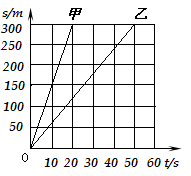
\includegraphics[scale=1]{figures/图片11.png} 


\question
如下图所示,量筒的直径$d$为\answerline*[1.20]$cm$。

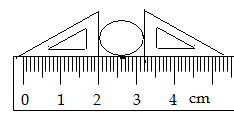
\includegraphics[scale=1]{figures/图片12.png} 


\question
如下图所示,是小球从静止开始下落时的频闪摄影照片。照相机拍照时每隔$0.02s$曝光一次。由照片可知,小球从A位置下落到F位置时所用的时间是\answerline*[0.1]$s$,此过程中,小球下落的平均速度大约是\answerline*[4]$m/s$。

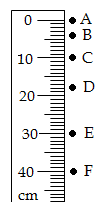
\includegraphics[scale=1]{figures/图片13.png} 


\question
小明同学在今年初中毕业升学体育考试$50m$跑项目中,取得$7s$的成绩。求:
\begin{enumerate}
\item 小明的平均速度;
\item 如果终点计时员听到发令枪才计时,则小明的成绩比他的实际成绩快多少秒?(已知声速为$340m/s$,结果保留两位小数。)
\end{enumerate}

\begin{solution}[10ex]
(1)$v=s/t=50m/s \approx 7.14m/s $

(2)由$v=s/t$ 得 $t_ \textrm{声}=s_\textrm{声}/v_\textrm{声}=50m/340m/s \approx 0.15s$
\end{solution}


\question
一座大桥长$1.6km$,一列长$200m$的火车以$15m/s$的速度通过此桥,火车完全通过此桥所需的时间为多少?

\begin{solution}[8ex]
解:S=S桥+S车      $t=s/v=(1600m+200m)/15m/s=120s$
\end{solution}

\end{questions}
\end{Aquestions}



\end{document}



